\begin{figure}[!ht]
	\centering
	\begin{subfigure}{0.32\linewidth}
			\centering
			\imagebox{0.9\linewidth}{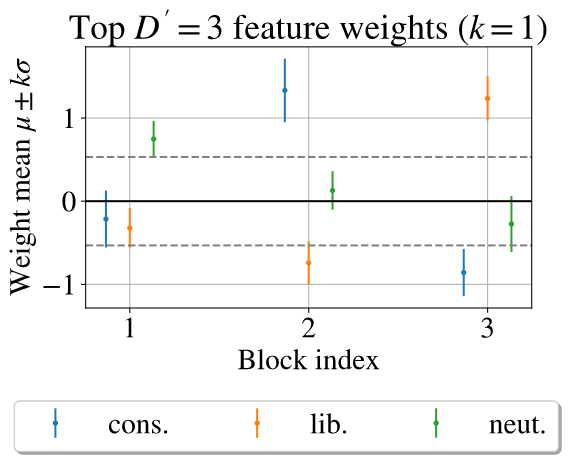
\includegraphics[width=\linewidth]{polbooks-null-1}}
			\caption{Political books}
			\label{fig:polbooks-null}
		\end{subfigure}
	\begin{subfigure}{0.32\linewidth}
			\centering
			\imagebox{0.9\linewidth}{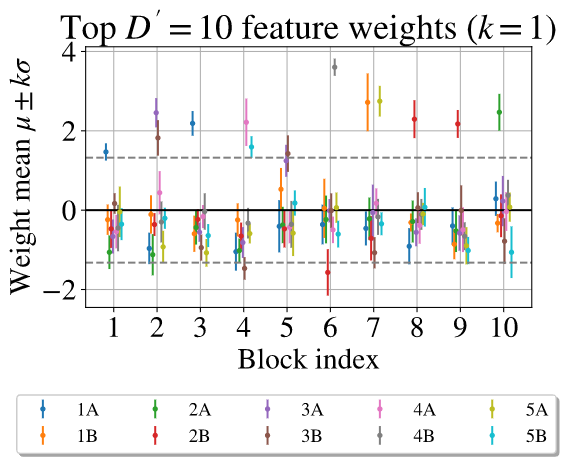
\includegraphics[width=\linewidth]{school-null-1}}
			\caption{Primary school}
			\label{fig:school-null}
		\end{subfigure}
	\begin{subfigure}{0.32\linewidth}
			\centering
			\imagebox{0.9\linewidth}{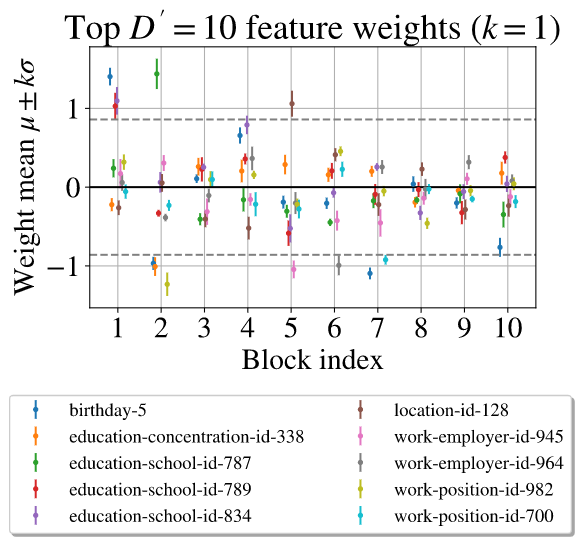
\includegraphics[width=\linewidth]{fb-null-1}}
			\caption{Facebook egonet}
			\label{fig:fb-null}
		\end{subfigure}
	\caption{Top $D'$ $\theta$-samples for each dataset. Coarse steps on x-axis give block index and the fine steps denote give index. Dotted line is $\pm c^*$.}
\end{figure}
%
\begin{figure}[!ht]
	\centering
	\begin{subfigure}{0.32\linewidth}
			\centering
			\imagebox{0.8\linewidth}{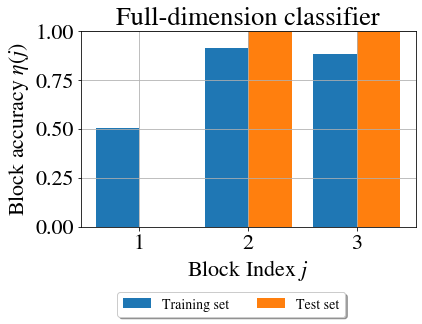
\includegraphics[width=\linewidth]{polbooks-accuracy-2}}
			\caption{Political books}
			\label{fig:polbooks-accuracy}
		\end{subfigure}
	\begin{subfigure}{0.32\linewidth}
			\centering
			\imagebox{0.8\linewidth}{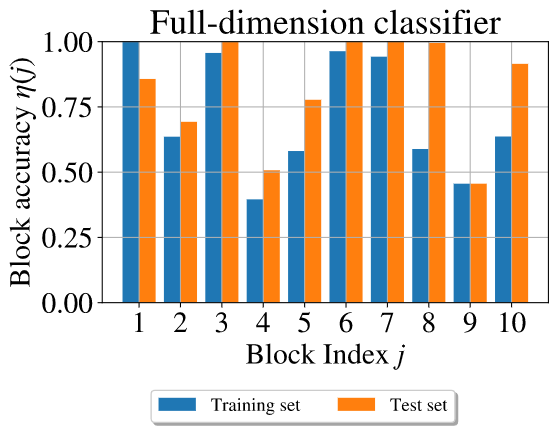
\includegraphics[width=\linewidth]{school-accuracy-1}}
			\caption{Primary school}
			\label{fig:school-accuracy}
		\end{subfigure}
	\begin{subfigure}{0.32\linewidth}
			\centering
			\imagebox{0.8\linewidth}{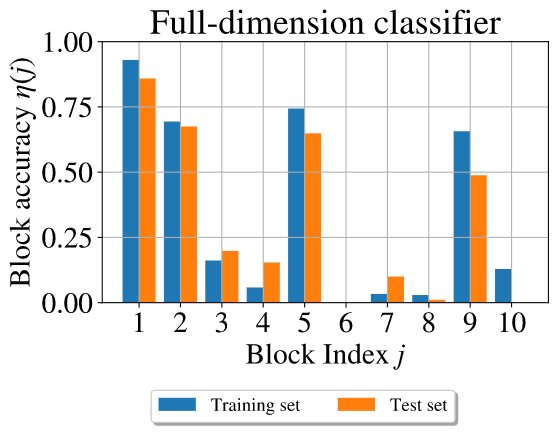
\includegraphics[width=\linewidth]{fb-accuracy-1}}
			\caption{Facebook egonet}
			\label{fig:fb-accuracy}
		\end{subfigure}
	\caption{Per-block accuracy $\eta(j)$ for each dataset.}
\end{figure}